\subsection{Giá trị cực đại và cực tiểu}
Đạo hàm có một ứng dụng quan trọng trong việc xác định các \textbf{cực đại địa phương} và \textbf{cực tiểu địa phương}. Trước hết, ta sẽ tìm hiểu về hai khái niệm này.
\begin{definition}
    \textbf{Cực đại địa phương} của hàm số \(f(x)\) tại điểm \(x=a\) là giá trị \(f(a)\) nếu tồn tại một khoảng mở \((a-\delta, a+\delta)\) với \(\delta > 0\) sao cho:
    \[
    f(a) \geq f(x) \quad \forall x \in (a-\delta, a+\delta)
    \]
\end{definition}
\begin{definition}
    \textbf{Cực tiểu địa phương} của hàm số \(f(x)\) tại điểm \(x=a\) là giá trị \(f(a)\) nếu tồn tại một khoảng mở \((a-\delta, a+\delta)\) với \(\delta > 0\) sao cho:
    \[
    f(a) \leq f(x) \quad \forall x \in (a-\delta, a+\delta)
    \]
\end{definition}
Và các điểm trên được gọi chung là \textbf{cực trị} của hàm số \(f(x)\).
\begin{figure}[H]
\centering
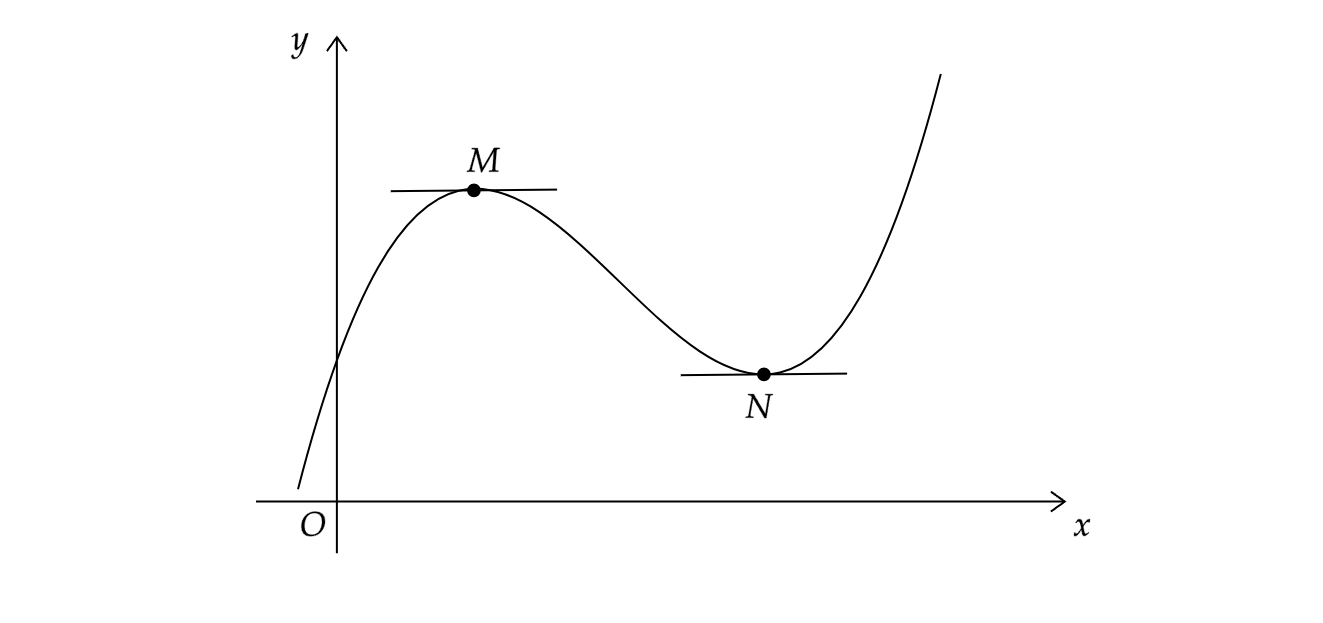
\includegraphics[width=0.8\textwidth]{Tuan1/ảnh/cuctri.png}
\caption{Cực đại địa phương (điểm \(M\)) và cực tiểu địa phương (điểm \(N\))}
\end{figure}
Từ hình vẽ trên, ta có thể thấy tại các điểm cực trị, tiếp tuyến của đồ thị nằm ngang. Từ đó, ta có định lý sau:
\begin{theorem}
    \textbf{Định lý Fermat}: Nếu hàm số \(f\) có cực trị tại \(a\), thì \(f'(a)=0\) nếu đạo hàm này tồn tại.
\end{theorem}
Tuy nhiên, định lý đảo của định lý trên không đúng.
\begin{figure}[H]
\centering
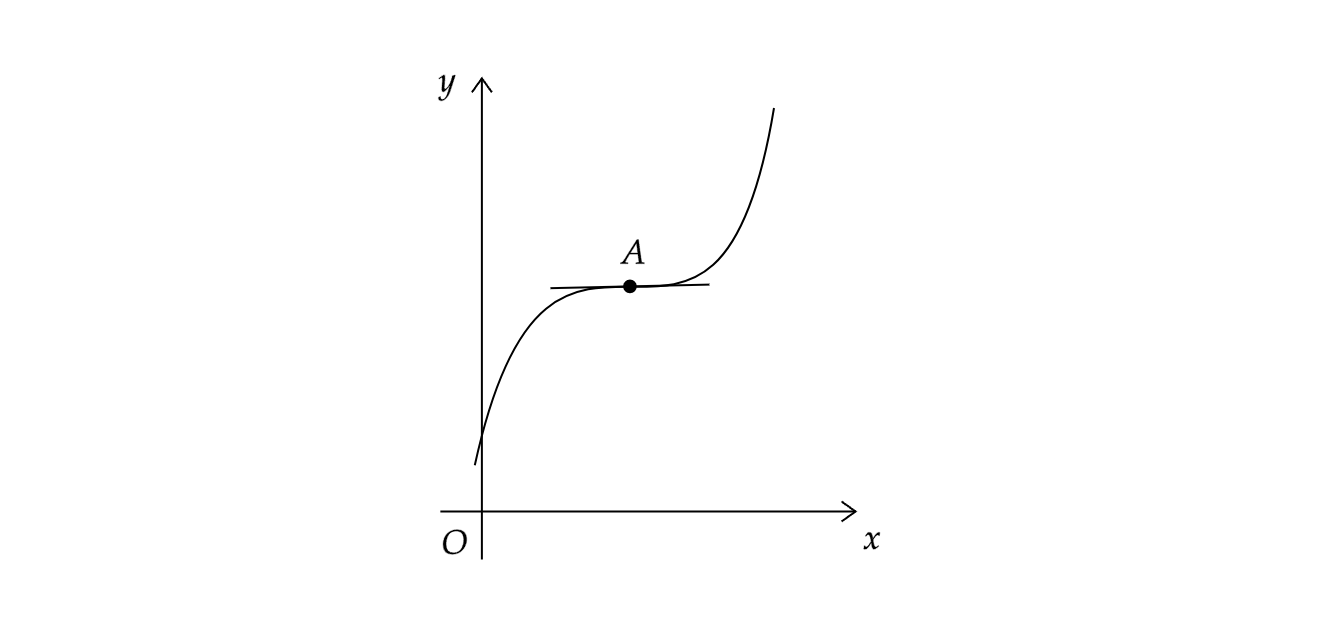
\includegraphics[width=0.8\textwidth]{Tuan1/ảnh/khongcuctri.png}
\caption{Điểm uốn \(A\) của đồ thị hàm số}
\end{figure}
Từ hình vẽ trên, ta có thể thấy đạo hàm của hàm số tại điểm \(A\) bằng 0 nhưng đây không phải là điểm cực trị. Điểm này được gọi là \textbf{điểm uốn} của đồ thị hàm số.

Một cách để xác định điểm cực trị là cực đại hay cực tiểu địa phương là sử dụng định lý sau:
\begin{theorem}
    Xét hàm \(f\) có đạo hàm bằng 0 tại điểm \(a\), nếu:
    \begin{itemize}
    \item \(f''(a) > 0\), thì \(f(a)\) là cực tiểu địa phương.
    \item \(f''(a) < 0\), thì \(f(a)\) là cực đại địa phương.
    \end{itemize}
\end{theorem}
Nếu \(f''(a) = 0\), ta không thể kết luận được gì về điểm này. Trong trường hợp đó, ta sẽ cần sử dụng các phương pháp sẽ được bàn luận trong các bài tập...

\subsection{Định lý giá trị trung bình}
Định lý giá trị trung bình là một trong những định lý quan trọng của giải tích. Nhưng trước khi đến với định lý này, ta sẽ cần giới thiệu một định lý khác:
\begin{theorem}
\textbf{Định lý Rolle}: Nếu hàm số \(f\) là liên tục và khả vi trên khoảng \([a, b]\), và \(f(a) = f(b)\), thì tồn tại ít nhất một điểm \(c \in (a, b)\) sao cho \(f'(c) = 0\).
\end{theorem}
Chúng ta có thể nhìn vào đồ thị của các hàm số thỏa mãn điều kiện trên để thấy được ý nghĩa trực quan của điểm \(c\):
\begin{figure}[H]
\centering
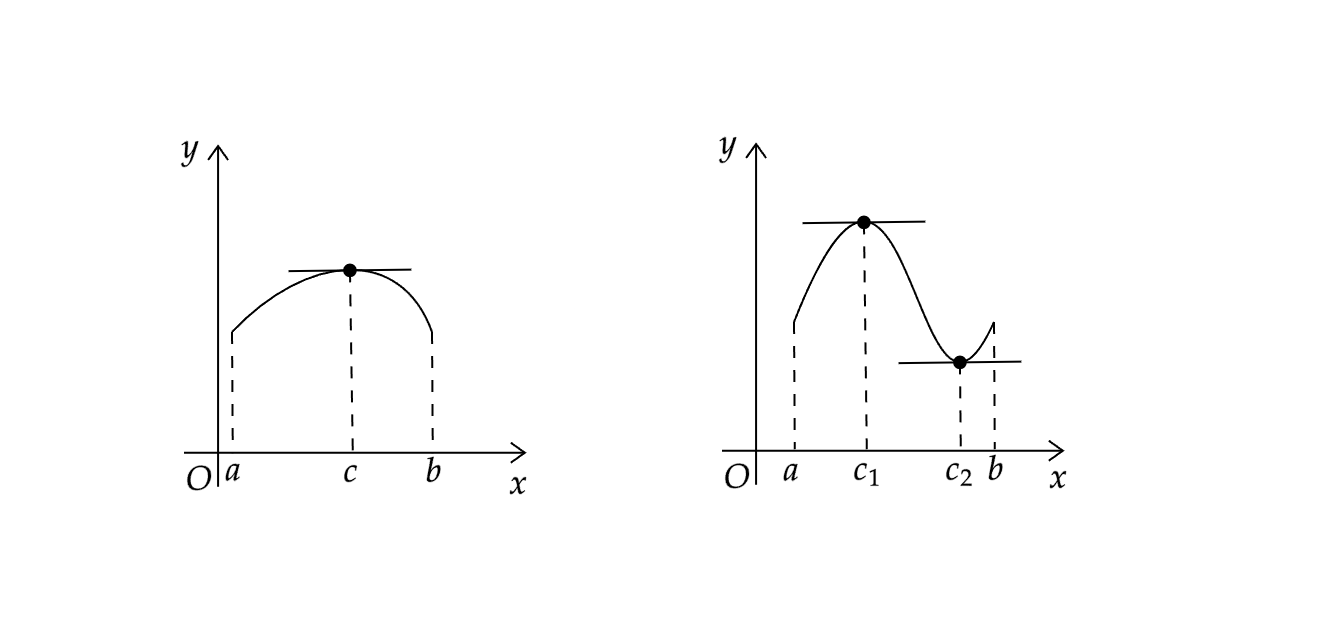
\includegraphics[width=0.8\textwidth]{Tuan1/ảnh/ĐL Rolle.png}
\caption{Định lý Rolle}
\end{figure}
Việc chứng minh chặt chẽ sẽ là nhiệm vụ của bạn trong bài tập....

Định lý giá trị trung bình là một mở rộng của định lý Rolle. Định lý này phát biểu như sau:
\begin{theorem}
\textbf{Định lý giá trị trung bình}: Nếu hàm số \(f\) là liên tục và khả vi trên khoảng \([a, b]\), thì tồn tại ít nhất một điểm \(c \in (a, b)\) sao cho:
\begin{equation}
f'(c)=\frac{f(b) - f(a)}{b - a}
\end{equation}
hay
\begin{equation}
f(b) - f(a) = f'(c)(b - a)
\end{equation}
\end{theorem}
Khi này, độ dốc của tiếp tuyến tại điểm \(c\) bằng với độ dốc của cát tuyến nối giữa hai điểm \(a\) và \(b\):
\begin{figure}[H]
\centering
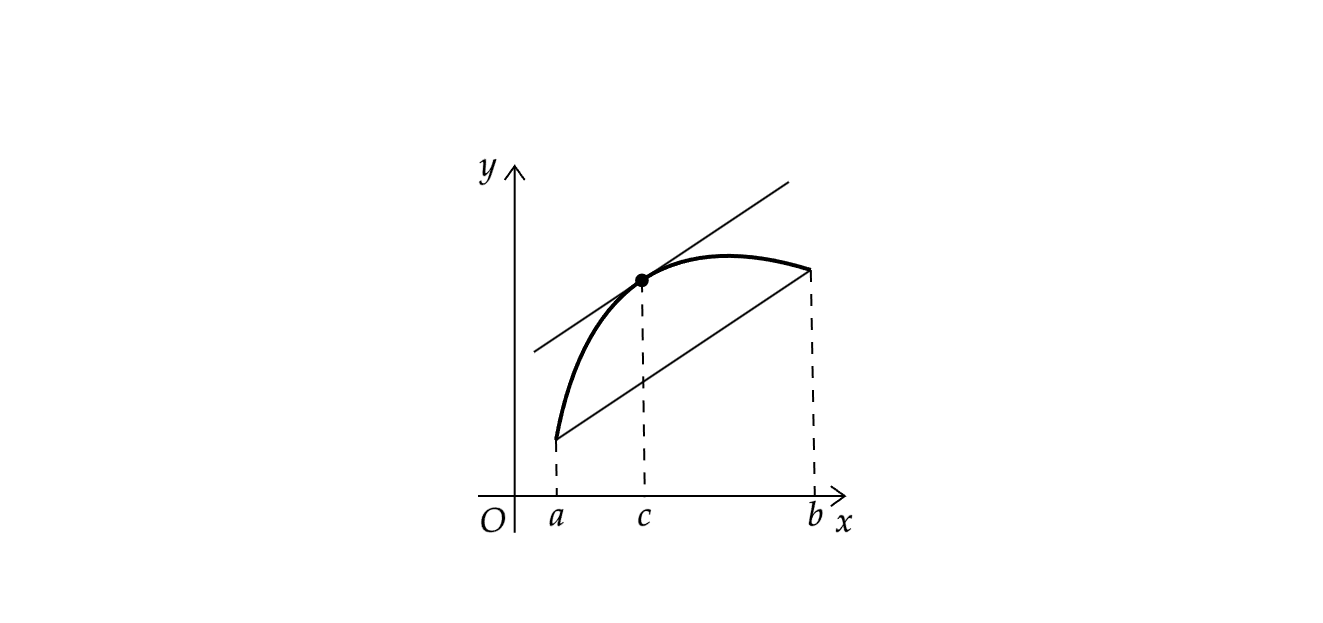
\includegraphics[width=0.8\textwidth]{Tuan1/ảnh/ĐL GTTB.png}
\caption{Định lý giá trị trung bình}
\end{figure}
Chứng minh định lý này sẽ là nhiệm vụ của bạn trong bài tập....
\subsection{Xấp xỉ đa thức của hàm số}
Trong thực tế, chúng ta thường cần tính giá trị của một hàm số tại một điểm nào đó. Tuy nhiên, việc tính toán trực tiếp có thể phức tạp hoặc không khả thi. Do đó, chúng ta thường sử dụng các đa thức xấp xỉ để ước lượng giá trị của hàm số.
\begin{theorem}
Nếu \(f\) có một khai triển bằng chuỗi lũy thừa tại \(a\), tức là nếu
\begin{equation}
f(x)=\Sigma_{n=0}^{\infty}c_n(x-a)^n
\end{equation}
thì các hệ số của nó được cho bởi công thức sau
\begin{equation}
c_n=\frac{f^{(n)}(a)}{n!}
\end{equation}
trong đó \(f^{(n)}(a)\) là đạo hàm bậc \(n\) của hàm số \(f\) tại điểm \(a\).

Chuỗi lũy thừa này được gọi là \textbf{chuỗi Taylor} của hàm số \(f\) tại điểm \(a\).
\end{theorem}
Khi ta chỉ lấy một vài số hạng của chuỗi, ta thu được một phép xấp xỉ:
\begin{definition}
\textbf{Khai triển Taylor bậc \(n\)} của hàm số \(f\) tại điểm \(a\):
\begin{equation}
f(x)\approx f(a)+f'(a)(x-a)+\frac{f''(a)}{2!}(x-a)^2+\cdots+\frac{f^{(n)}(a)}{n!}(x-a)^n
\end{equation}
\end{definition}
Càng lấy tới bậc càng cao, độ chính xác của phép xấp xỉ càng cao.